
\begin{figure*}[tbh]
  \begin{center}
%    \subfigure[Mean download rate]{\label{fig:allisps_mean_throughputs}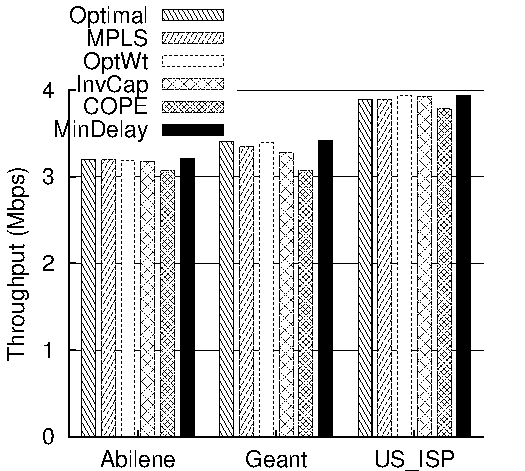
\includegraphics[width=35mm,height=30mm]{final_images/mean_throughput_hist_plot.pdf}}
    \subfigure{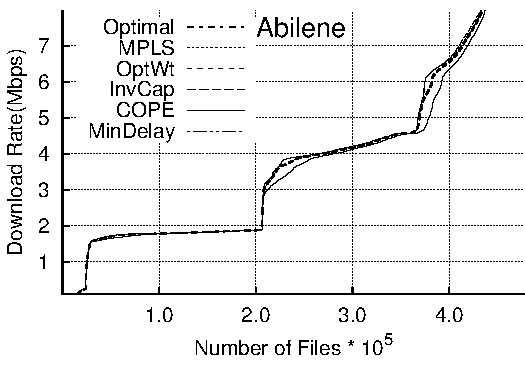
\includegraphics[scale=0.55]{final_images/G3_CDF/Abilene_download_rates_aggregate_plot.pdf}}
    \subfigure{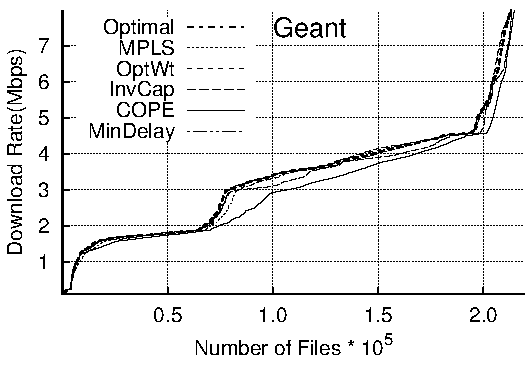
\includegraphics[scale=0.55]{final_images/G3_CDF/Geant_download_rates_aggregate_plot.pdf}}
    \subfigure{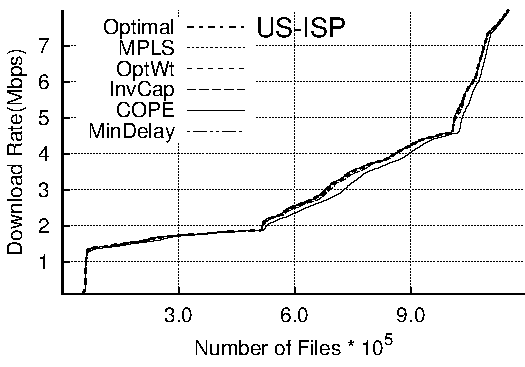
\includegraphics[scale=0.55]{final_images/G3_CDF/ATT_download_rates_aggregate_plot.pdf}}

  \end{center} 
  \caption{Download rate CDFs for all TE schemes are near identical except \cope\ which has slightly lower performance}
  \label{fig:throughputs_CDF}
\end{figure*}

\section{User-perceived performance}
\label{sec:app_performance}
In this section, we present a comparative analysis of the impact of different TE schemes on user-perceived performance. A summary of our findings is as follows. First, all TE schemes  including \invcap\ show nearly identical user-perceived performance for TCP and UDP traffic. Second, different TE schemes do achieve different MLUs as expected, suggesting that MLU is a poor predictor of user-perceived performance. Third, COPE consistently performs slightly worse than all other schemes in TCP throughput, suggesting that accounting for unpredictable variations in traffic hurts the common case user-perceived performance.

%we present our comparison of traffic engineering schemes based on simulation of traffic matrices at Internet loads for 3 ISPs. Our simulation shows that unexpectedly that all traffic engineering schemes (even \invcap) perform near identical in terms of download rates using TCP for all ISPs. We also show that MLU a metric commonly used metric for traffic engineering does not predict TCP throughput well and traffic engineering which optimizes for unexpected traffic variations increases delay and hurts TCP throughput.

%In this section, we present our comparison of traffic engineering schemes based on simulation of traffic matrices at Internet loads for 3 ISPs. Our simulation shows that unexpectedly that all traffic engineering schemes (even \invcap) perform near identical in terms of download rates using TCP for all ISPs. We also show that MLU a metric commonly used metric for traffic engineering does not predict TCP throughput well and traffic engineering which optimizes for unexpected traffic variations increases delay and hurts TCP throughput.

%Prior works on traffic engineering have measured its performance using linear programming simulation and have used metrics such as the maximum link utilization or similar cost functions based on link utilization.


\subsection{TCP performance}

We simulate TMs from 2 days of data for each ISP. For each day, we simulated 50 matrices measured at 5-minute intervals for Abilene, 25 matrices measured at 15-minute intervals for Geant, and 24 matrices measured hourly for US-ISP. We present results for the second day. The metric of user-perceived performance is the \emph{download rate} of files using TCP, where the file arrival workload is generated using the traffic matrices as described in Section \ref{sec:sim_TM}.

%\begin{figure}
%\begin{center}
%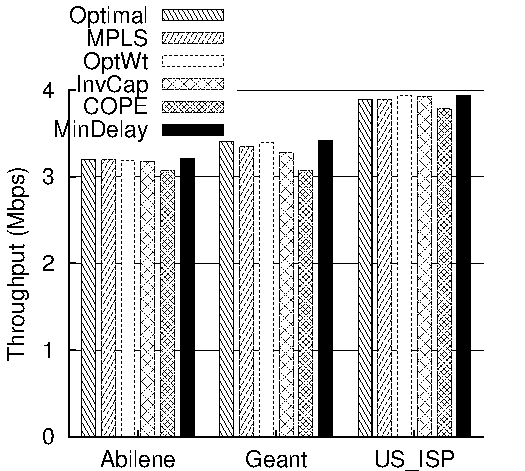
\includegraphics[scale=0.6]{final_images/mean_throughput_hist_plot.pdf}
%\caption{Mean download rates}
%\end{center}
%\label{fig:allisps_mean_throughputs}
%\end{figure}
%
%\begin{figure}
% \begin{center}
%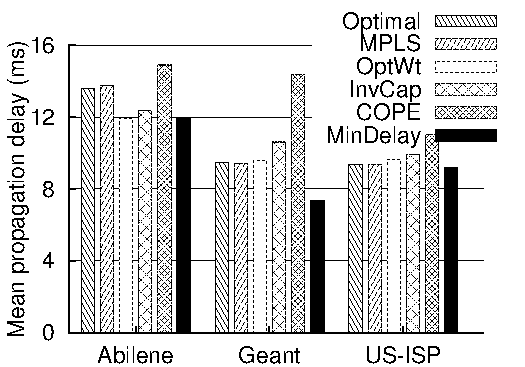
\includegraphics[scale=0.6]{final_images/G4_propdelay/mean_prop_delay_plot.pdf}
%\caption{COPE has the highest propagation delay among TE schemes}
% \end{center}
% \label{fig:prop_delay_all}
% \end{figure}


Figure \ref{fig:allisps_mean_throughputs} shows the mean download rate of files, where the average is across all files across all of the simulated matrices for each TE scheme.
We make three observations from this graph. 
First, all schemes achieve nearly same mean download rates with the exception of COPE that is consistently worse by up to  10\%.
Next, \opt\ (the leftmost bar in each group) is not always the best as minimizing MLU is not the same as optimizing TCP performance.
Finally,  \mindelay\ (the leftmost bar in each group) that optimizes latency performs the same as other TE schemes that optimize link utilization based metrics.


Figure \ref{fig:throughputs_CDF} shows the corresponding CDFs for the mean download rates in Figure \ref{fig:allisps_mean_throughputs}. The CDFs show that the near-identical TCP performance achieved by all TE schemes is not an artifact of presenting a specific statistic such as the mean, but is reflected by the entire distribution.  All distributions show a stepwise increase which suggests that access links are a bottleneck for a significant fraction of file transfers. This observation partly explains why \mindelay\ fails to  improve TCP throughput over other schemes: TCP throughput cannot be improved for flows bottlenecked at access link even if \mindelay\ scheme reduced the RTT for these flows.

\begin{figure*}[t]
\begin{minipage}{0.45\textwidth}
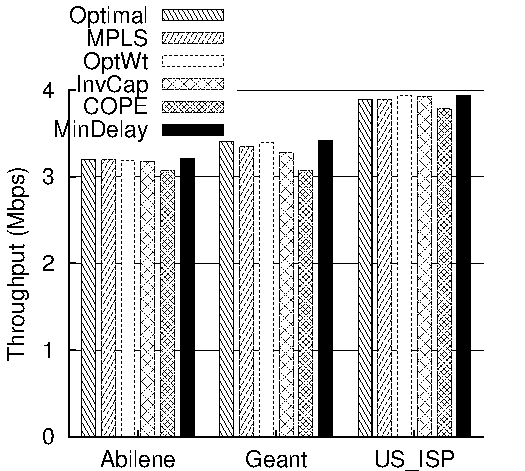
\includegraphics[scale=0.6]{final_images/mean_throughput_hist_plot.pdf}
\caption{Mean download rates}
\label{fig:allisps_mean_throughputs}
\end{minipage}
\hspace{1cm}
\begin{minipage}{0.45\textwidth}
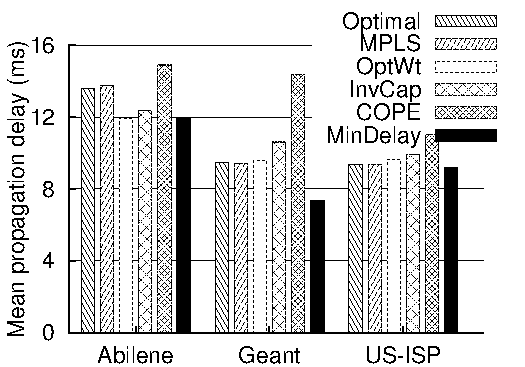
\includegraphics[scale=0.6]{final_images/G4_propdelay/mean_prop_delay_plot.pdf}
\caption{COPE has the highest propagation delay among TE schemes}
 \label{fig:prop_delay_all}
\end{minipage}
\end{figure*}

% we present the download rate of all files from all traffic matrices during the day sorted in increasing order  and in Figure ~\ref{fig:allisps_mean_throughputs} we show the mean value of the above distribution.

%What is result ?
%The download rate curves for all traffic engineering schemes are strikingly similar for all the topologies. Even the simple routing scheme, \invcap{}  has mean and median throughputs within 5\% of \opt{}  for all 3 topologies.  \opt{} does not have any additional gain over other routing schemes in download rate. The only notable difference is throughput is for \cope{} which has up to 10\% lower median throughput than \opt{} for Geant toplogy and has lowest throughput among all schemes. All 3 graphs show a step-wise increase which shows that access link are bottleneck for a significant fraction of file transfers.


%
%\begin{figure}[htb]
%  \begin{center}
%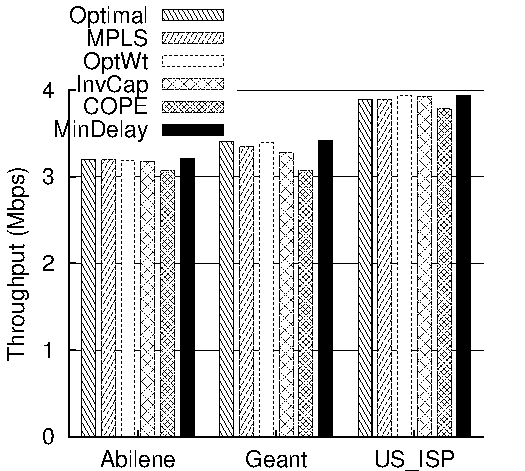
\includegraphics[scale=0.5]{final_images/mean_throughput_hist_plot.pdf}
% \end{center}
%	  \caption{Mean download rates of files for Internet traffic matrices}
%  \label{fig:allisps_mean_throughputs}
%\end{figure}




%\begin{figure*}[tbh]
%  \begin{center}
%%    \subfigure[Mean download rate]{\label{fig:allisps_mean_throughputs}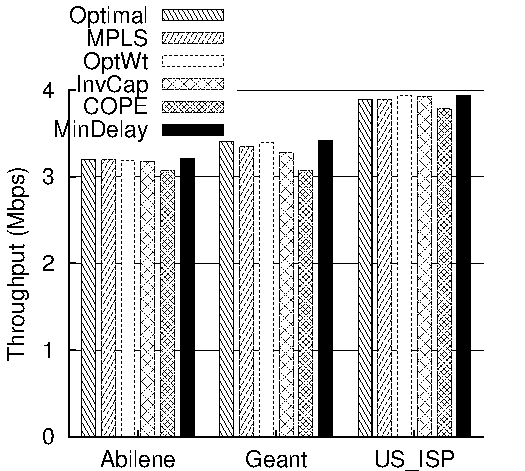
\includegraphics[width=35mm,height=30mm]{final_images/mean_throughput_hist_plot.pdf}}
%    \subfigure[Download rate CDF Abilene]{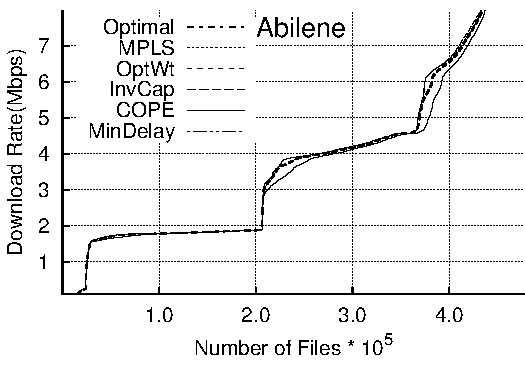
\includegraphics[scale=0.6]{final_images/G3_CDF/Abilene_download_rates_aggregate_plot.pdf}}
%    \subfigure[Download rate CDF Geant]{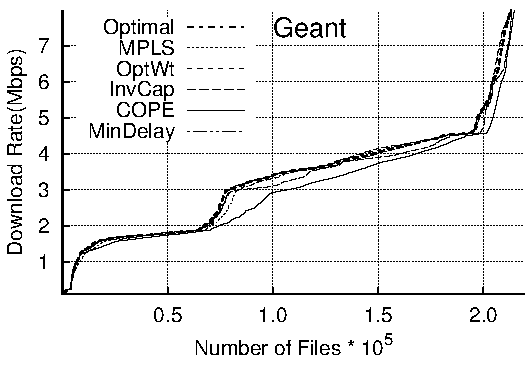
\includegraphics[scale=0.6]{final_images/G3_CDF/Geant_download_rates_aggregate_plot.pdf}}
%    \subfigure[Download rate CDF US-ISP]{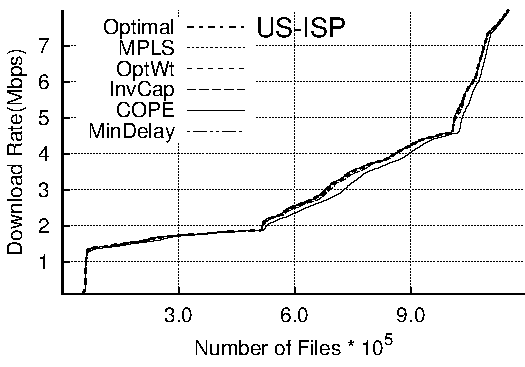
\includegraphics[scale=0.6]{final_images/G3_CDF/ATT_download_rates_aggregate_plot.pdf}}
%  \caption{Download rate CDFs for all TE schmes are near identical except \cope\ which has slightly lower performance}
%  \label{fig:throughputs_CDF}
%  \end{center} 
%\vspace{-0.2in}
%\end{figure*}

%\subsection{Analysis}
%Here, we present an analysis of above results using additional statistics measured from simulation.

\subsubsection{MLU vs. TCP performance}

To further investigate the results in Figure \ref{fig:allisps_mean_throughputs} and Figure \ref{fig:throughputs_CDF}, we analyze the empirically observed MLU for all TE schemes in the experiments. Figure \ref{fig:All_ISPs_MLU} plots the MLUs for all matrices considered. For US-ISP the MLU data is proprietary, so we present the ratio of MLU with respect to \opt. As expected, different TE schemes do show substantially different MLUs. For example, the MLU for \invcap\ and \optwt\ is up to twice the MLU of \opt\ in some cases; \mindelay\ has a MLU of 0.6 on Geant, which is more than twice of \opt's MLU. These results suggest that MLU is a poor predictor of download rate performance: schemes with near-identical TCP throughput have very different MLUs, and COPE despite achieving near-optimal MLU consistently shows sub-optimal TCP throughput.

%\textbf{MLU:}
%The above results may seem surprising if we observe the empirical MLU of all the traffic matrices simulated (Figure ~\ref{fig:All_ISPs_MLU}). The graphs show a significant difference among traffic engineering schemes. MLU for \invcap{} or \optwt{} is up to twice the MLU of \opt{} in many cases. The contrast between MLU and download rate graphs leads us to the conclusion that a higher MLU for Internet traffic matrices does not imply a worse TCP performance. We observe that \cope{} has a MLU close to \opt{} in Geant and US-ISP topologies but its download rate is lower than all other TE schemes. This is because \cope{} has greater path delay. This shows that even a low MLU traffic engineering scheme can have a worse TCP performance.

The main reason why MLU does not affect download rate is because queuing delay and loss rates are negligible until link utilization reaches a threshold. In our experiments, link utilization below 0.7 causes near negligible loss rates and queuing delays. Since the MLUs on most of the traffic matrices are below this value, loss rates on backbone links minimally impact the throughput of file downloads.  These observations are consistent with a recent  study on Level-3 ISP network  \cite{ExpRouterBuffer} showing that loss rates on backbone links are zero even at 95\%  link utilization. This threshold is expected to be higher for actual backbone traffic as our experiments are at scale 1/10 or smaller. At larger scales, there would be more concurrent flows resulting in less bursty traffic and lower loss rates.

%The main reason why MLU does not affect download rate is because queuing delay and loss rates are negligible until link utilization reaches a threshold. We observe this in our simulation and this phenomenon has also been observed for backbone traffic in the Internet \cite{ExpRouterBuffer}. Since the MLUs on most of the traffic matrices are below this threshold, loss rates on backbone links minimally impact the throughput of file downloads.  These observations are consistent with a recent study on Level-3 network\cite{ExpRouterBuffer} showing that loss rates on backbone links are zero even at 95\%  link utilization. In our simulations, the threshold at which links exhibit non-negligible loss is around 0.7. This threshold is expected to be higher for actual backbone traffic as our experiments are at scale 1/10 or smaller. At larger scales, there would be more concurrent flows resulting in less bursty traffic and lower loss rates.


The second reason why MLU hardly impacts the average download rate as well as the distribution is because it is largely determined by the traffic of only one link. Even under high MLU, the rest of the network may not be congested. File download rates are affected only for flows on this link, which may be a tiny fraction of the total traffic.




%There may exist intermittent traffic congestion which cause higher loss rates on backbone links. These happen due to interdomain routing changes \cite{BGPloss} (which are frequent) or due to anomalous traffic spikes in the Internet. An intradomain TE protocol cannot gurard against losses due to interdomain routing changes. It can be argued that doing \opt{} TE (using online traffic engineering) or a  TE scheme similar to \cope{} which is robust to traffic fluctuations would perform better in case of traffic spikes. These two routing schemes do not show any gain compared to other offline traffic engineering schemes in our experiment.  We infer that either these spikes are short enough to affect the average traffic matrices measured in our data set or the ISP networks are well provisioned to handle the spikes.


%\begin{figure}[tbh]
%  \begin{center}
%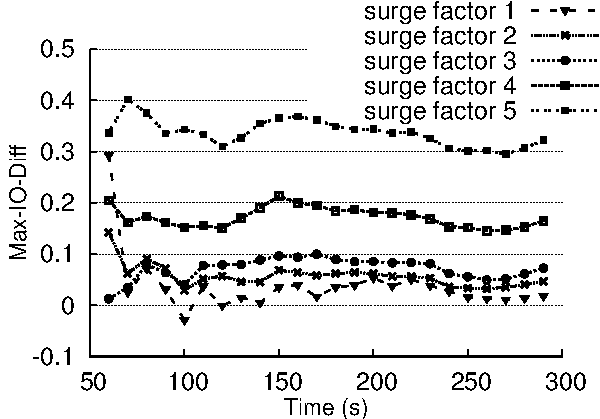
\includegraphics[scale=0.6]{final_images/G4_propdelay/i_o_diff_plot.pdf}
%  \end{center}
%  \caption{Propagation delay for Internet TMs.}
%  \label{fig:prop_delay_all}
%\end{figure}



\begin{figure*}[tb]

  \begin{center}
\subfigure{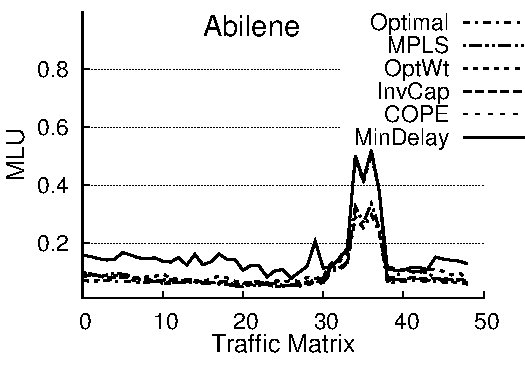
\includegraphics[scale=0.55]{final_images/G2_MLU//Abilene_MLUAverageUtilTable_plot.pdf}}
\subfigure{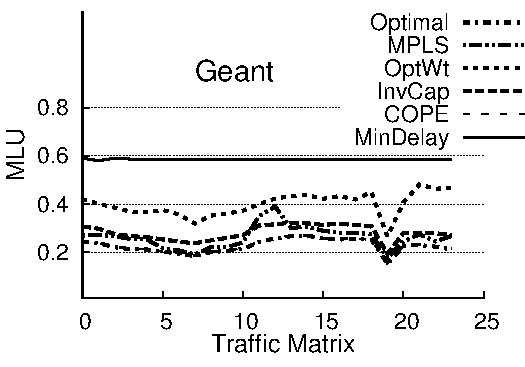
\includegraphics[scale=0.55]{final_images/G2_MLU//Geant_MLUAverageUtilTable_plot.pdf}}
\subfigure{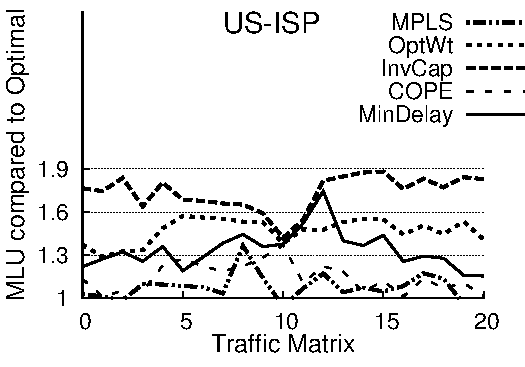
\includegraphics[scale=0.55]{final_images/G2_MLU//ATT_MLUAverageUtilTable_plot.pdf}}
  \end{center}
  \caption{TE schemes differ as much as 2$\times$ in MLU}
  \label{fig:All_ISPs_MLU}
  \end{figure*}
  
  
 
%\begin{minipage}{1.9in}
%  \begin{center}
%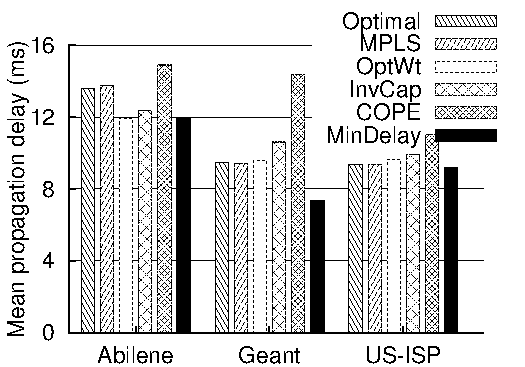
\includegraphics[scale=0.6]{final_images/G4_propdelay/mean_prop_delay_plot.pdf}
%  \end{center}
%  \caption{}
%
%
%  \label{}
%\end{minipage}
%\vspace{-0.2in}


\subsubsection{The price of predictability}
Why is \cope's performance consistently worse than the other schemes? To investigate this, we analyzed the propagation delays of routes computed by COPE. Given uniformly low loss rates and queueing delays, propagation delays primarily determine TCP performance.

Figure \ref{fig:prop_delay_all} shows the path delay averaged across all files and across all matrices for the different TE schemes. \cope{} has a significantly higher delay compared to all other schemes. We attribute this phenomenon to \cope{}'s optimization approach, which engineers for unpredictable spikes in traffic demands. Specifically, \cope\ attempts to bound the worst-case MLU for any traffic matrix similar to oblivious routing like schemes \cite{Cohen}. \cope\ intentionally routes some traffic along longer paths so as to leave room for occasional traffic spikes along shorter paths. While this approach makes \cope\ robust with respect to MLU under rare spikes in traffic, it comes at the cost of hurting common-case user-perceived performance.  Although we have not experimented with other oblivious routing schemes, these results suggest that any oblivious routing scheme that attempts to optimize MLU, e.g., \cite{Cohen}, is likely to incur a similar penalty in  user-perceived performance in the common case. 

%Although prior work has recognized that TE schemes can increase path delay, e.g.. \cite{TeXCP06}, to the best of our knowledge, our work is the first to empirically quantify the impact on TCP throughput and to show that engineering for rare traffic spikes comes at the cost of hurting common-case TCP throughput.

%It is known that TE schemes can increase path delay \cite{TeXCP06}. Our contributions are to show that \cope\ has a significantly higher path delay than other TE schemes and  to accurately measure the impact of increased path delay on TCP throughput. 


%This statistic explains why \cope{} has the lowest download rate among all schemes for Geant and US-ISP topologies. Our finding also suggests that other oblivious routing schemes which optimize for MLU \cite{ObliviousRouting} may have lower TCP throughput.

%We infer that the robustness of \cope to unpredictable traffic spikes comes at the cost of higher path delay and reduced TCP througput.  


%We observe that in Geant and US-ISP topologies \cope has lower mean and median value than other schemes. It is because the routing computed by \cope has a higher path delay compared to other traffic engineering schemes. We show the average propagation delay for all TE schemes in ~\ref{fig:prop_delay_all}. This statistic is the average of propagation delay of each file in our simulation. Different routings have same file request sequence but their paths depend on the routing. All TE schemes except \cope have similar path delay. The higher delay is significant for Geant and US-ISP topologies which explains its lower throughput. 

%\textbf{Users' Access Link Capacity:}

%Access link capacity is the  bottleneck for majority of file downloads in Figure ~\ref{fig:throughputs_CDF} but this may not hold true in Internet. The reasons are that paths have more delay (e.g. intercontinenal links), the access link at the server may be a bottleneck. Both these observations  affect all TE schemes identically and are unlikely to affect our findings. 

%It may be argued that our findings would not hold if Internet users had higher access link capacities. To verify this hypothesis, we also performed experiments where users access links had twice the current access link capacities. Our results remained unchanged  \cite{TechReport}.


%The minimum value of download rate in Figure ~\ref{fig:throughputs_CDF} is near zero in our simulation. This is because of congestion at the access link of users. In some cases a new file download starts on the same user node before previous download has finished. The previous flow has a large window size and sends many more packets than the new flow. In some cases, this causes multiple packet losses	 at access link queue for the new flow. Repeated timeouts due to these loss result in near zero download rates for some files. 

% Summary of result
%In this section we presented our comparison of traffic engineering schemes for file download rates in Internet. Our novel simulation based comparison has following main results: (1) All traffic engineering schemes (even \invcap{}) performs near identical in file download rate for Internet traffic matrices. (2) MLU is a poor predictor of TCP throughput : \invcap{} which has 2x higher MLU than \opt has nearly the same throughput and \cope{}'s MLU is near optimal but its throughput is lowest. (3) A traffic engineering approach such as \cope{} which engineers for unpredictable traffic demands increases path delay and reduces TCP throughput.

\subsection{UDP performance}
\label{sec:UDP_perf}
\subsubsection{Measuring UDP performance}

We assume that the loss rate and the queuing delay on each link for UDP traffic is the same as that measured during experiments with TCP traffic. This assumption is reasonable as TCP accounts for over 90\% of Internet traffic \cite{SprintBackbone}. We calculate the loss rate and delay for a path by combining the loss rates of links along the path; we compute the delay by summing the propagation and queuing delay of links along the path.

We compare performance of VoIP traffic (which uses UDP) using Mean Opinion Score (MOS). MOS is an industry standard VoIP call quality metric for which a score of above 4 is considered good and below 3 is considered bad. We calculate MOS using the formula in \cite{MOS-formula}  which calculates MOS given the loss rate and delay for a path. 

We calculate MOS for VoIP calls between all pairs of source and destination PoP nodes in an ISP. First, we measure loss rates and queuing delay on backbone links for each 10-second interval.  For each interval, we calculate the MOS for a path based on its end-to-end loss rate and delay. The mean MOS for a path is the average value of MOS over all intervals. For TE schemes that split traffic across multiple paths between a source-destination pair, the mean MOS for a source-destination node pair is calculated as the weighted average of mean MOS weighted by the fraction of the traffic split along each path between the node pair. We similarly calculate the 5th percentile MOS for a source-destination pair by taking the weighted average of 5th percentile MOS values for all its paths.

\subsubsection{Results}
We obtain a distribution of mean MOS values for a TE scheme by combining mean MOS values for all pairs of source and destination nodes for all traffic matrices. We find that the minimum and the maximum values of mean MOS for all TE schemes are in the range (4.08, 4.14) for Abilene, (4.07, 4.14) for Geant and (4.08, 4.14) for US-ISP.  The range of values for 5th percentile MOS are (4.07, 4.13) for Abilene, (4.08, 4.14) for Geant and (4.05, 4.14) for US-ISP. MOS scores for all schemes are always above 4.0 and the differences between different TE schemes is at most 0.1. These results are not surprising since loss rates and queuing delay are near-negligible for most links in the network. Furthermore, MOS is not very sensitive to few milliseconds difference in propagation delay among TE schemes.




%\tbd{In summary, our study of the impact of state-of-the-art TE schemes on application performance reveals the following. All TE schemes have near-identical TCP throughput and UDP performance for a VoIP call quality metric. }

	


%The only exception is \cope\ that has a slightly lower TCP throughput, which is because it attempts to absorb unpredictable variations in traffic at the cost of common case application performance. Furthermore, we find that the commonly used MLU metric is a poor predictor of TCP performance. Taken together, these results suggest that the simplest routing scheme, \invcap, suffices to achieve similar performance as sophisticated traffic engineering schemes proposed in the literature or in use in production networks today.

%Our experiments in this section showed that all traffic engineering schemes perform near identical in terms of TCP throughput for traffic matrices from 3 ISPs in the Internet. Even though traffic engineering schemes differ by as much as twice in terms of MLU, their TCP throughput is identical because of near zero loss rates and queuing delay on most links. An interesting observation is that \cope which has MLU close to \opt has a lower TCP throughput.

%In the following section, we experiment with traffic matrices at higher load than current Internet and study the effect of application adaptation.


%In FIgure ~\ref{fig:All_ISPs_MLU} we show the maximum link utlization for the traffic matrices we experiment with. The graphs show a significant difference among traffic engineering schemes. MLU for \invcap or \optwt being upto twice the MLU of \opt but these differences are not reflected in throughputs. Higher link utliizations cause increased loss rates and higher queuing delay for packets. We find that in our experiments both these values remain near-zero until link utilization values of 0.6 in our experiments. Since the MLU on most of the traffic matrices are below this threshold value, MLU isnt a factor in the throughput of file downloads. Even if the utilization on one link is high enough to increase loss rates on that link the rest of the network may not be facing any congestion. File downloads rates are affected only for flows on this link, which could a small fraction of total traffic.


%In Fig ~\ref{fig:allisps_aggregate_InternetBW}, we also show the CDF of TCP throughput for all files for US-ISP topology . This shows that access link is the bottleneck for a large fraction of file transfers in our simulation. This helps us explain the near identical values for all routings. This observation is likely to be different for internet since paths have more delay (e.g. intercontinenal links ), the access link at the server may be a bottleneck, and there may exist intermittent traffic congestion which cause higher loss rates on backbone links. The first two reasons affect all TE schemes identically and are unlikely to affect our findings. The third reason intermittent congestion on backbone in internet can happen beacuse of interdomain routing changes [cite sprint study] ( which are frequent ) or due to anomalous traffic spikes in the internet. An intra domain TE protocol cannot gurard against losses due to interdomain routing changes. It can be argued that doing \opt TE ( using online traffic engineering ) or a  TE scheme similar to \cope which is robust to traffic fluctuations would perform better in case of traffic spikes. Since these two routing schemes do not show an improvement compared to other offline traffic engineering schemes, either these spikes are short enough to affect the average traffic matrix over 15 min or 1 hour period or the spikes do not cause performance degradation for internet traffic matrices for all TE schemes.


%It must be noted that our experiments are at scale 1:10 to 1:50. At, higher scale the loss rate and queuing delay would be lower at the same link utilization level. As scale increases, the router buffer sizes increase and the per packet processing time decrease proportionally. If we take the analogy from a queuing model such as $M/M/1/K$ queue, at higher loads the mean packet arrival rate ($\lambda$), the mean packet processing rate($\mu$) and the capacity of the queue ($K$) increase proportionately. The formula for loss rates of this queuing model show that both these metrics decrase as $\lambda$, $\mu$  and $K$ increase proportioately \cite{queue}. If anything , the scale of our experiments reinforces our results that MLU has minimal application performance in realistic ISP topologies. 


%\subsubsection{Comparison of path delay}
%
%In Fig ~\ref{fig:prop_delay_all}, we present the average propagation delay for TE methods. The propagation delays presented are the average propagation delay for all file transfers.  The notable outlier in the table is \cope which has the highest delay in all three topologies. It delay is maximum in Geant where it has 25\% higher delay than the next highest delay TE method. This explains the the reason for \cope having lower throughput than other TE schemes. All other TE methods have delay within 1ms of each other for Abilene and US-ISP. Their near identical througputs reflect this trend.
%
%We calculate this statistic from the traffic matrix and routing computed by a TE method. First, we calculate the delay of tranfers between a source destination pair by multiplying the propagation delay by the total traffic on each path. The sum of this delay for all source destination pairs gives the total delay for a traffic matrix. The total propagation delay is the sum of delays of all trafic matrices divided by the sum of all traffic matrices.


%
%\begin{figure}
%\begin{center}
%  \begin{tabular}{| l | c | c | c | }
%    \hline
%Routing & Abilene & Geant & US-ISP \\ \hline \hline
%\opt &  4.54 &	9.46 & 9.37\\ \hline
%\invcap & 4.13 &10.62 & 9.90 \\ \hline
%\mplsavg & 4.58 & 9.40 & 9.37\\ \hline
%\cope &4.97 & 14.38 & 11.03\\ \hline
%\optwt & 3.98 & 9.57 & 9.64\\ \hline
%MinDelay & 3.97 & 7.34 & 9.21\\ \hline
%  \end{tabular}
%\caption{Propagation delay (in ms) for TE methods on different topologies}
%\end{center}
%\label{fig:prop_delay_all}
%\end{figure}

%\subsection{Effect of access link bottlenecks}
%
%We measure the effect of access link capcity of users on our results by experimenting at higher capacity access link bottlenecks. A reasonable choice for higher access link bottleneck is doubling current the access link capacities. In Table ~\ref{fig:all_isps_internetBWx2} shows the mean throughputs for all 3 ISPs. The mean throghputs increase by 1.3-1.7 times but the relative difference between different routings remain the same. This shows that throughputs of different traffic engineering schmes are near identical because of current traffic load in the network and would remain identical even if the current internet bandwidths were much higher.
%
%\begin{figure}[tbh]
%  \begin{center}
%\includegraphics[scale=0.7]{newImages/mean_throughput_twice_internetBW.jpg}
%  \end{center}
%  \caption{Mean throughputs of file transfers at twice internet access link bandwidths}
%  \label{fig:all_isps_internetBWx2}
%\end{figure}

%\begin{figure}
%\begin{center}
%  \begin{tabular}{| l | c | c | c | }
%\hline
%Routing & Abilene & Geant & US-ISP \\ \hline \hline			
%\opt	&	589.5	&	720.6	&	671.1	\\ \hline
%\\invcap	&	580.6	&	721.9	&	640.1	\\ \hline
%\mplsavg	&	589.4	&	720.0	&	654.1	\\ \hline
%\cope	&	560.4	&	695.4	&	587.8	\\ \hline
%\optwt	&	586.2	&	723.1	&	662.2	\\ \hline
%MinDelay	&	589.8	&	723.9	&	663.9	\\ \hline
%  \end{tabular}
%\caption{Mean throughputs at twice the internet access link bottlenecks}
%\end{center}
%\label{fig:all_isps_internetBWx2}
%\end{figure}

%\begin{figure*}[htb]
%  \begin{center}
%    \subfigure[Download rate US-ISP]{\label{fig:edge-a}\includegraphics[scale=0.4]{newImages/US_ISP/internetBW_scale2/download_rates_aggregate_plot.pdf}} 
%    \subfigure[Download rate Geant ISP]{\label{fig:edge-a}\includegraphics[scale=0.4]{newImages/Geant/internetBW_scale2/download_rates_aggregate_plot.pdf}} 
%    \subfigure[Download rate Abilene ISP]{\label{fig:edge-a}\includegraphics[scale=0.4]{newImages/Abilene/internetBW_scale2/download_rates_aggregate_plot.pdf}}  
%    \subfigure[Download ratio US-ISP]{\label{fig:edge-b}\includegraphics[scale=0.4]{newImages/US_ISP/internetBW_scale2/opt_download_ratios_aggregate_plot.pdf}} 
%    \subfigure[Download ratio Geant ISP]{\label{fig:edge-b}\includegraphics[scale=0.4]{newImages/Geant/internetBW_scale2/opt_download_ratios_aggregate_plot.pdf}} 
%    \subfigure[Download ratio Abilene ISP]{\label{fig:edge-b}\includegraphics[scale=0.4]{newImages/Abilene/internetBW_scale2/opt_download_ratios_aggregate_plot.pdf}} 
%  \caption{US Tier 1 ISP, Aggregate performance on 1 day traffic matrices,twice today's internet access link bottleneck distribution }
%  \end{center}
%  \label{fig:allisps_aggregate_internetBWX2}
%\end{figure*}

%As an interesting aside, we present the results for no access link bottlenecks in Fig  ~\ref{fig:allisps_aggregate_nolimit} .
%
%\begin{figure*}[htb]
%  \begin{center}
%\subfigure[US-ISP]{\label{fig:edge-c}\includegraphics[scale=0.75]{newImages/ATT_nolimit_Download_ratio_aggregate_plot.pdf}}
%\subfigure[Geant]{\label{fig:edge-c}\includegraphics[scale=0.75]{newImages/Geant_nolimit_Download_ratio_aggregate_plot.pdf}}
%\subfigure[Abilene]{\label{fig:edge-c}\includegraphics[scale=0.75]{newImages/Abilene_nolimit_Download_ratio_aggregate_plot.pdf}}
%  \end{center}
%  \caption{All ISPs : Download ratios for 1 day traffic matrices, without access link bottlenecks}
%  \label{fig:allisps_aggregate_nolimit}
%\end{figure*}

%\subsection{Experiments at higher scale}
%As said previously in this section, our simulations at lower scale provide a more challenging environment for comparison. To experimentally validate our findings at a higher scale, we selected 5 traffic matrices from each ISP and repeated our simulation at a higher scale. We simulated Abilene and Geant topology at original scale and the US-ISP topology at scale 1:10. We present the aggregate download ratios for 5 traffic matrices for at scale 1:50 and scale 1:10. The download ratios curve highlight the difference between traffic engineering schmes more clearly. The shape of the curves look almost the same in both graphs. This shows that our results remain consistent even at higher scale.
%
%Thus our results for 3 ISPs based on ns-2 simulations show that under traffic conditions in the internet the throughput performance of all traffic engineering schemes differ are near identical. Our results are consistent even at higher acess link botttlenecks in the internet and on experiment at higher scale. These findings show that difference in MLU for TE schemes does not translate to an improvement in throughput in internet conditions. Propagation delay is a more important factor and traffic engineering schemes which increase propagation delay have lower throughputs. 

%
%\subsection{Application Performance at higher loads}
%
%\subsubsection{Single Download Location}
%
%\subsubsection{Multiple Download Downloads}
